\documentclass[tikz,border=4pt]{standalone}
\usepackage{amsmath,amssymb}

\begin{document}
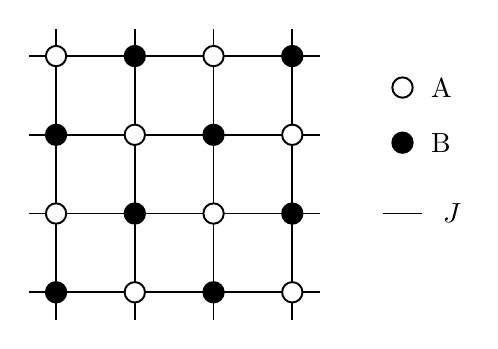
\begin{tikzpicture}[
  font=\normalsize,
  bond/.style={line width=0.6pt},
  siteA/.style={circle,draw=black,fill=white,line width=0.7pt,inner sep=2.6pt},
  siteB/.style={circle,draw=black,fill=black,line width=0.7pt,inner sep=2.6pt}
]
  % 4x4 square lattice
  \foreach \x in {0,1,2,3} {
    \draw[bond] (\x,-0.35) -- (\x,3.35);
    \draw[bond] (-0.35,\x) -- (3.35,\x);
  }
  \foreach \x in {0,1,2,3} {
    \foreach \y in {0,1,2,3} {
      \pgfmathtruncatemacro{\p}{mod(\x+\y,2)}
      \ifnum\p=1
        \node[siteA] at (\x,\y) {};
      \else
        \node[siteB] at (\x,\y) {};
      \fi
    }
  }
  % Legend (no Japanese text)
  \node[siteA] at (4.4,2.6) {};
  \node[right=4pt] at (4.5,2.6) {$\mathrm{A}$};
  \node[siteB] at (4.4,1.9) {};
  \node[right=4pt] at (4.5,1.9) {$\mathrm{B}$};
  \draw[bond] (4.15,1.0) -- (4.65,1.0);
  \node[right=4pt] at (4.65,1.0) {$J$};
\end{tikzpicture}
\end{document}
